% !TEX root = main.tex

% TODO:
% REMARK:

\section{Background Estimation}
\label{sec:BkgEst}

	According to the simulation, the events of interests occupy diminant ratio under signal region selection(includes $\chi^2_{min}$, MVA-A, MVA-B strategy), but also about 4$\sim$6 \% of events which came from non-$t\bar{t}$ background are collected. Even though the selected events are under high signal purity, the randomly combined background events would contaminate the final measurement of asymmetry. In fact, the minority of background may still dilute the calculating results of $A'_{cp}$ critically in this precision measurement analysis. Thus, the background study should be attached importance to. The $A'_{cp}$ value of $t\bar{t}$ would be extracted, at the same time, backgrounds' contribution would be cast aside.

	It is a common and usual way to estimate background in data by using simulation samples. It depends more on the theoretical modeling and detector simulation with simulation sample. The background in simulation cannot be quite close to real data perfectly. This situation would disorder the asymmetry measurement eventually. It is suggested that in many high energy experiments' analysis to directly acquire background from real data. Therefore, the data-driven way is applied.
	
	In this analysis, it is found that the $M_{lb}$ variable shows really difference between signal and background in shape(Fig.\ref{BkgEst:fig:SR_sigbkg_Mlbshape}). Thus, with the diverse shape, there is an advantage to discern signal and background and then seperate them with template fit.

		\begin{figure}[H]
		\centering
			\subfigure[$\chi^2_{min}$, mu-ch]{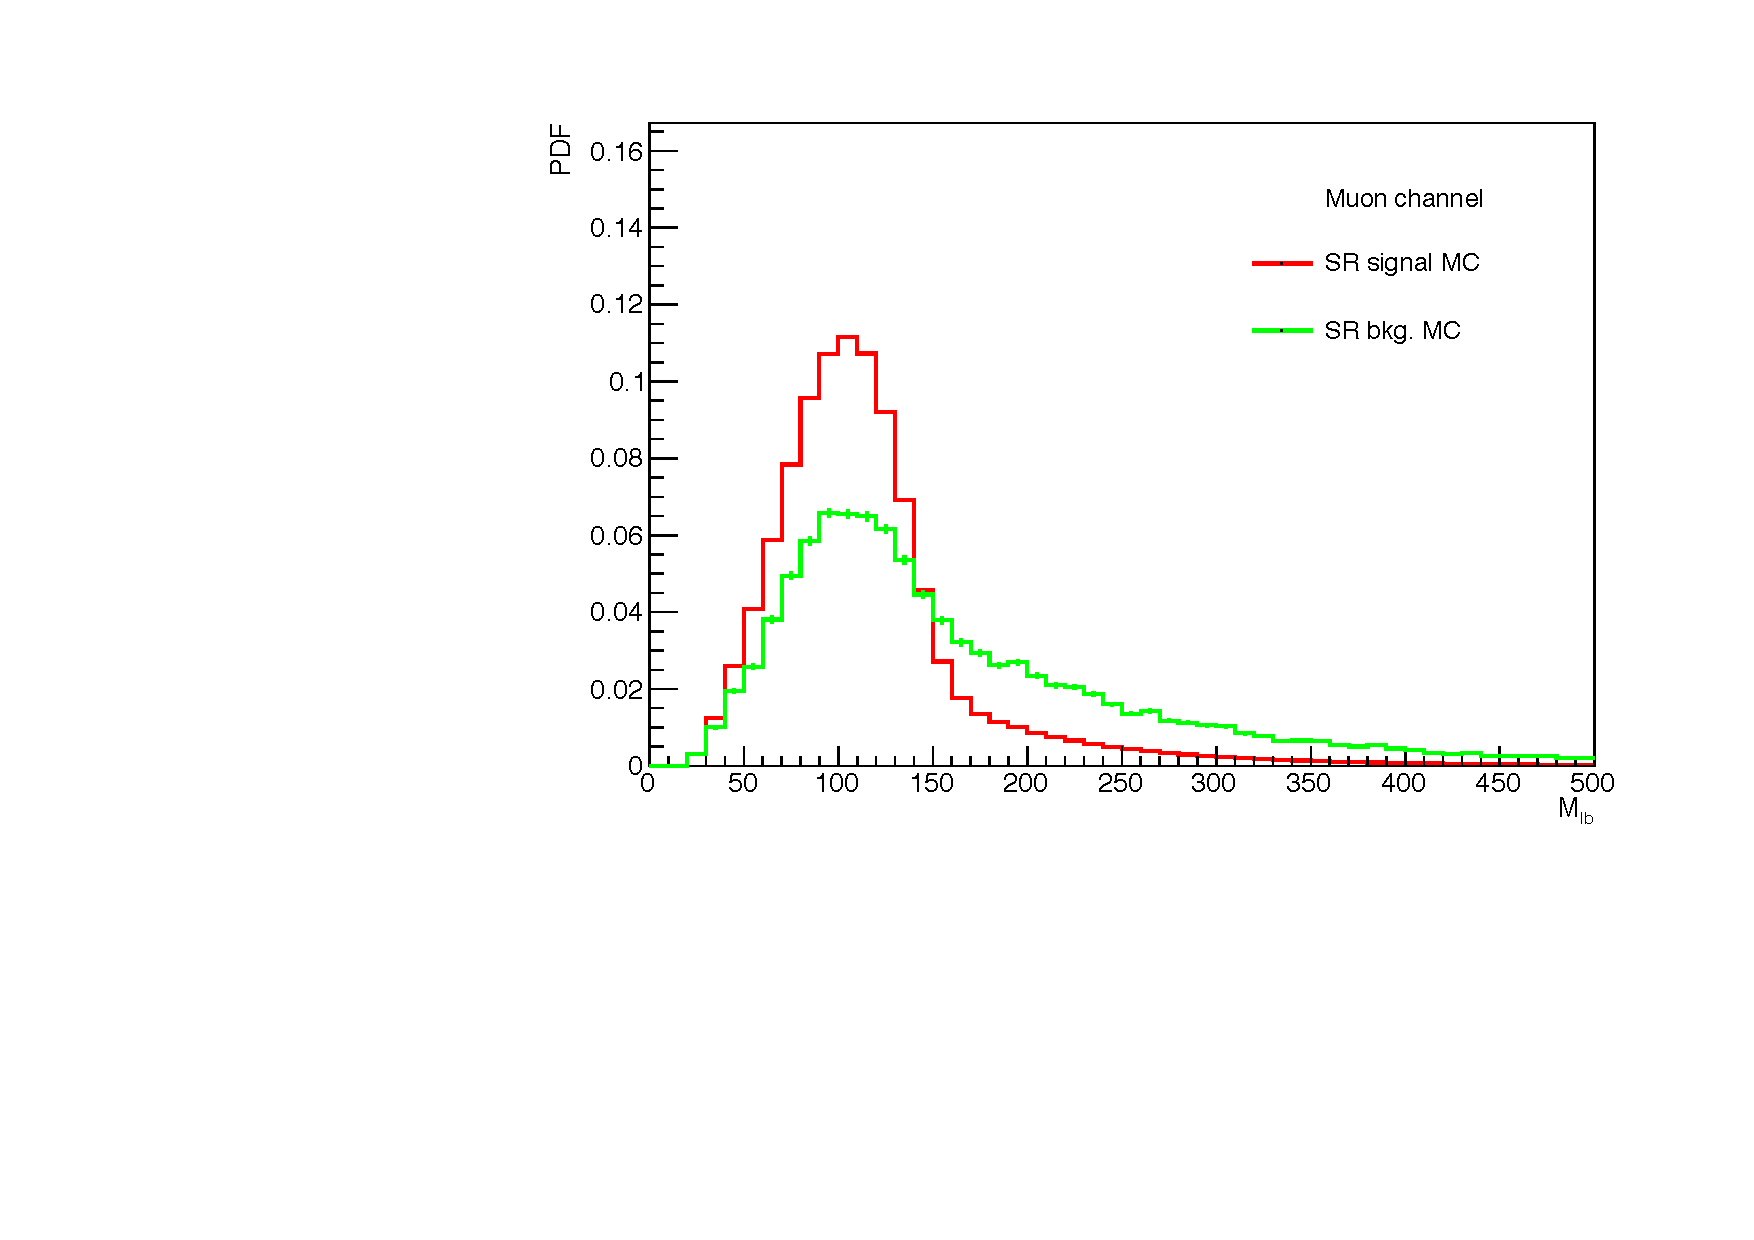
\includegraphics[width=0.45\textwidth]{Figures/BackgroundEstimation/chi2_SR_sig_bkg_shape_mu.pdf}}
			\subfigure[$\chi^2_{min}$, el-ch]{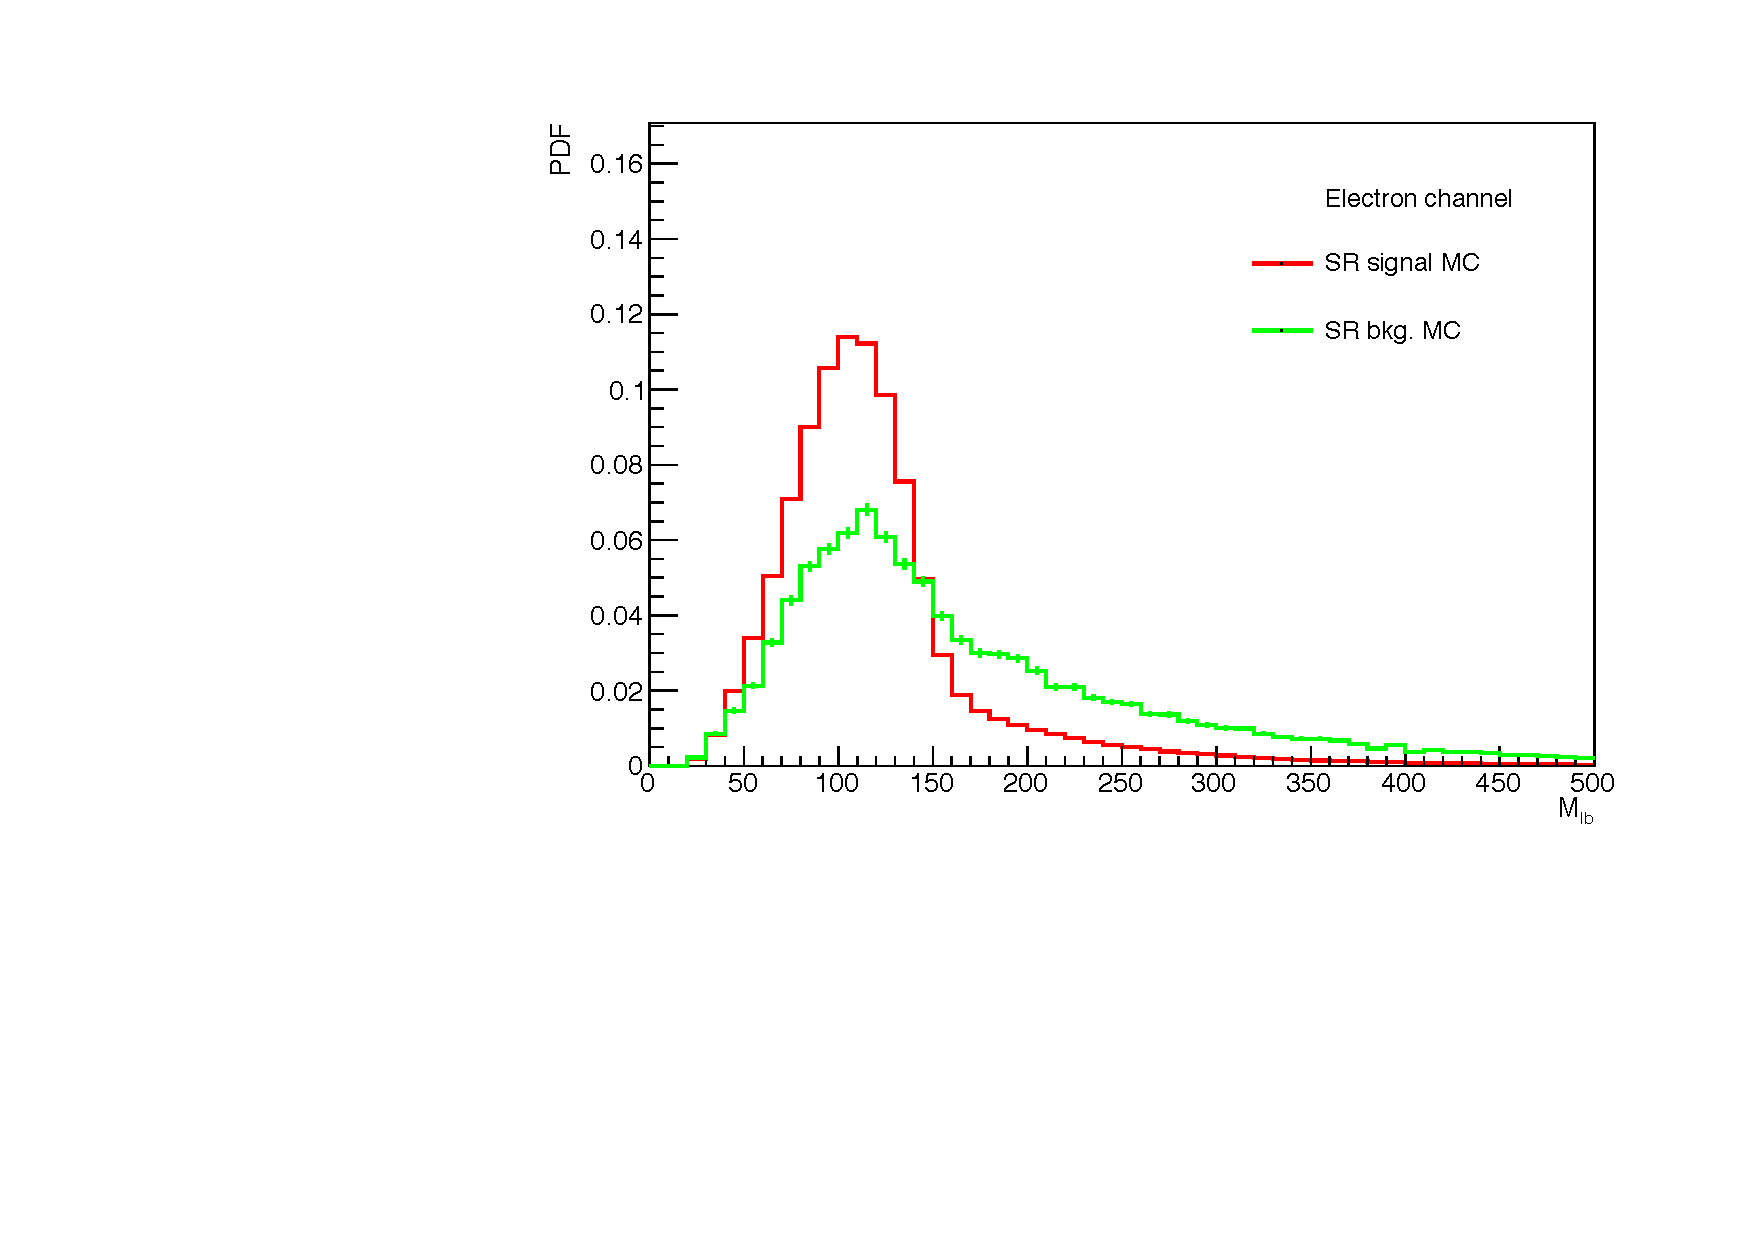
\includegraphics[width=0.45\textwidth]{Figures/BackgroundEstimation/chi2_SR_sig_bkg_shape_el.pdf}}\\
		\end{figure}
		\FloatBarrier
		\begin{figure}[H]
		\centering
			\subfigure[MVA(20 variables, MLP), mu-ch]{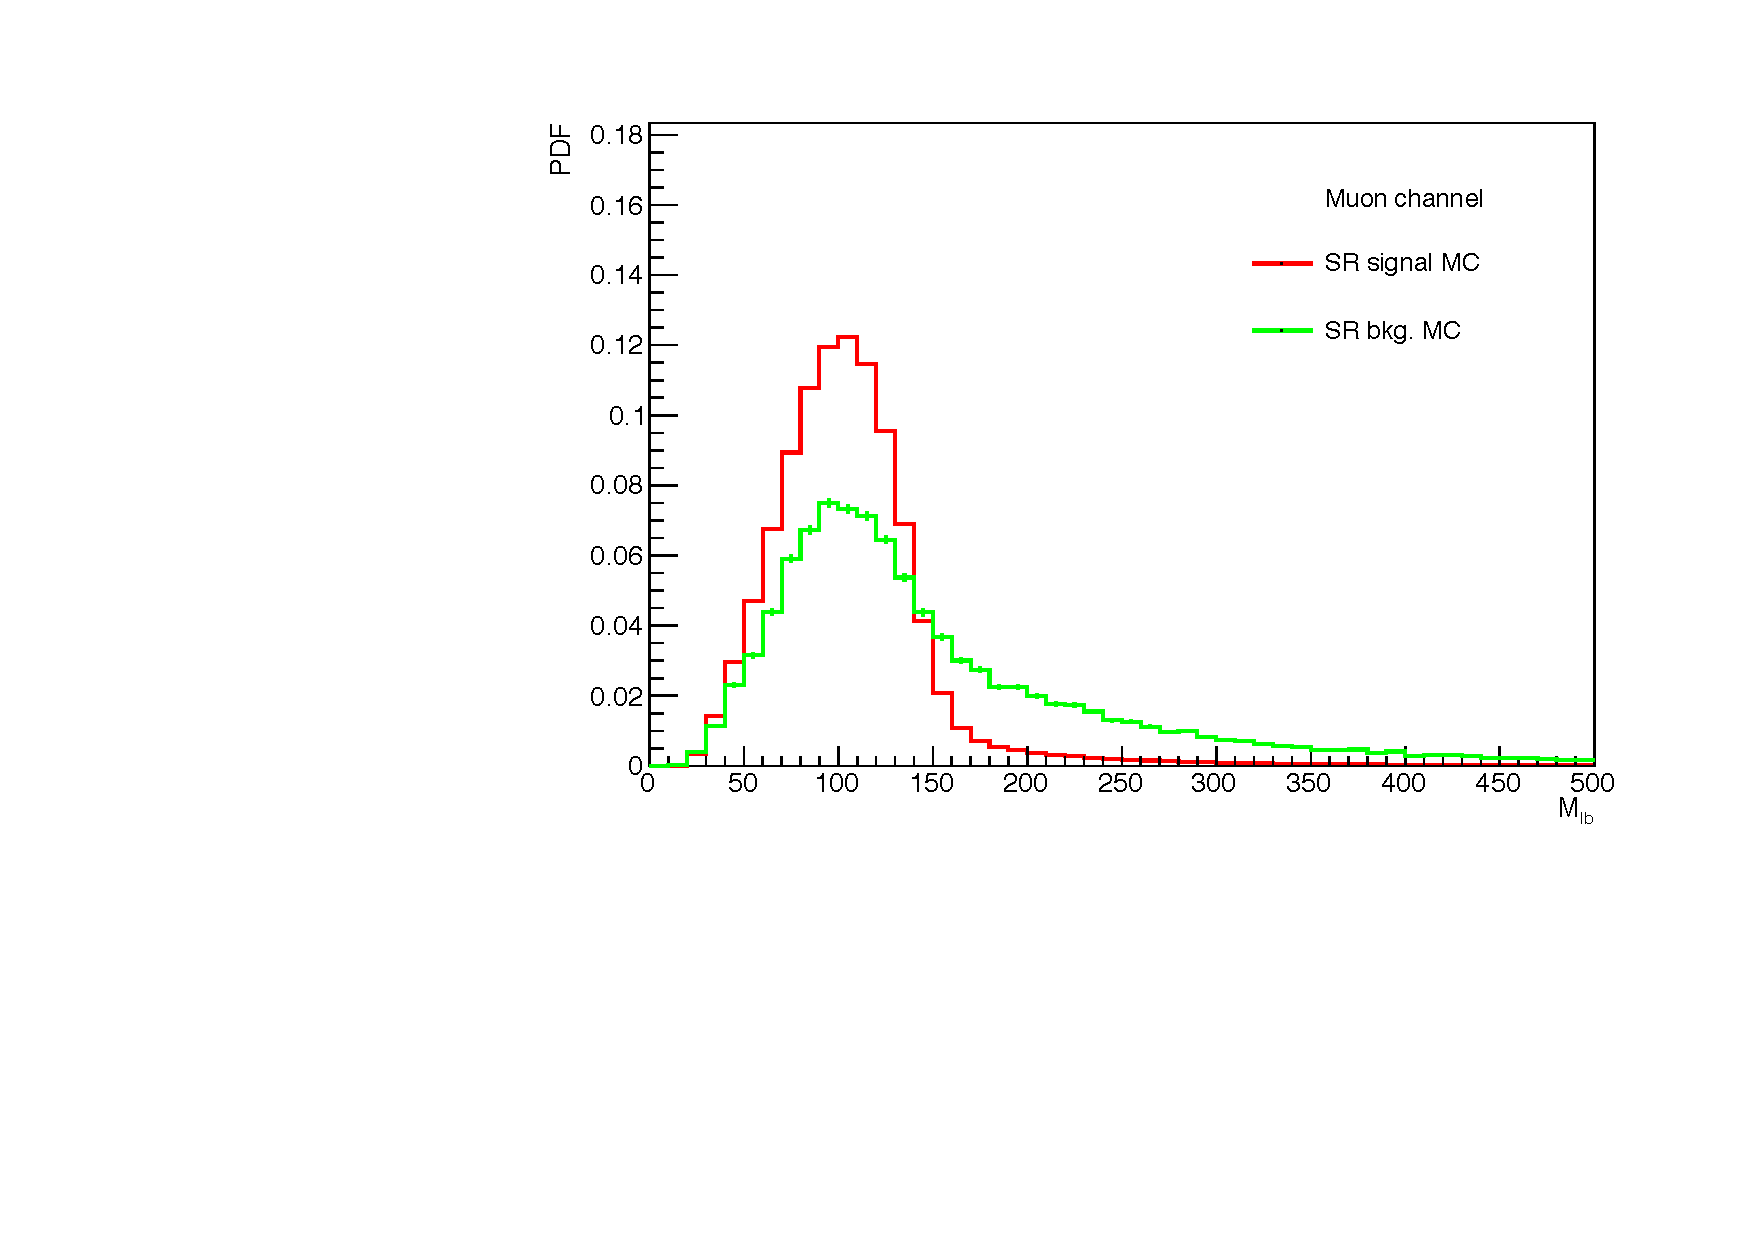
\includegraphics[width=0.45\textwidth]{Figures/BackgroundEstimation/a05_MLP_SR_sig_bkg_shape_mu.pdf}}
			\subfigure[MVA(20 variables, MLP), el-ch]{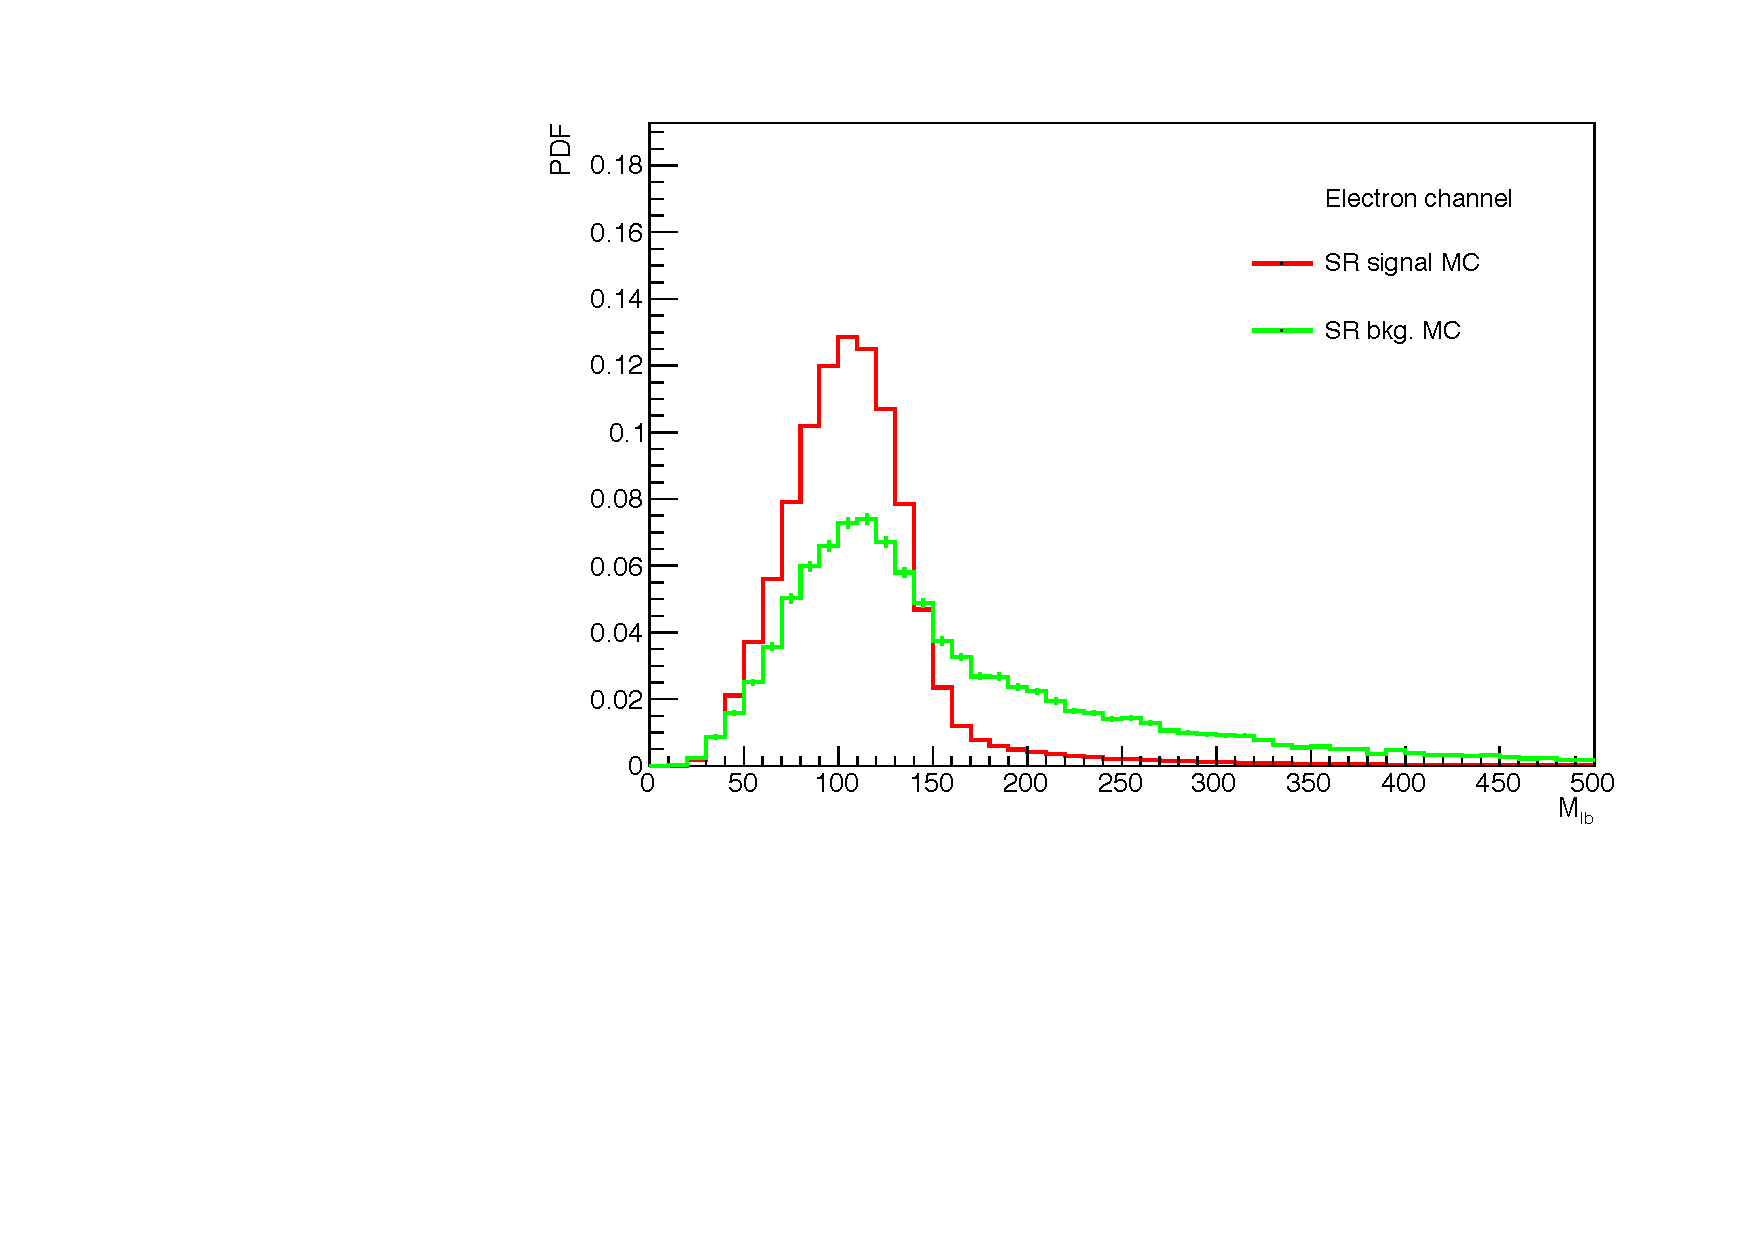
\includegraphics[width=0.45\textwidth]{Figures/BackgroundEstimation/a05_MLP_SR_sig_bkg_shape_el.pdf}}\\
		\caption{Comparison of $M_{lb}$ shape between SR's signal and background}
		\label{BkgEst:fig:SR_sigbkg_Mlbshape}
		\end{figure}
		\FloatBarrier

	As mentioned that the W+jets-dominant CR's data is used to data-driven background in SR, it must be checked that how the similarity of $M_{lb}$'s pdf shape they have:

		\begin{figure}[H]
		\centering
			\subfigure[$\chi^2_{min}$, mu-ch]{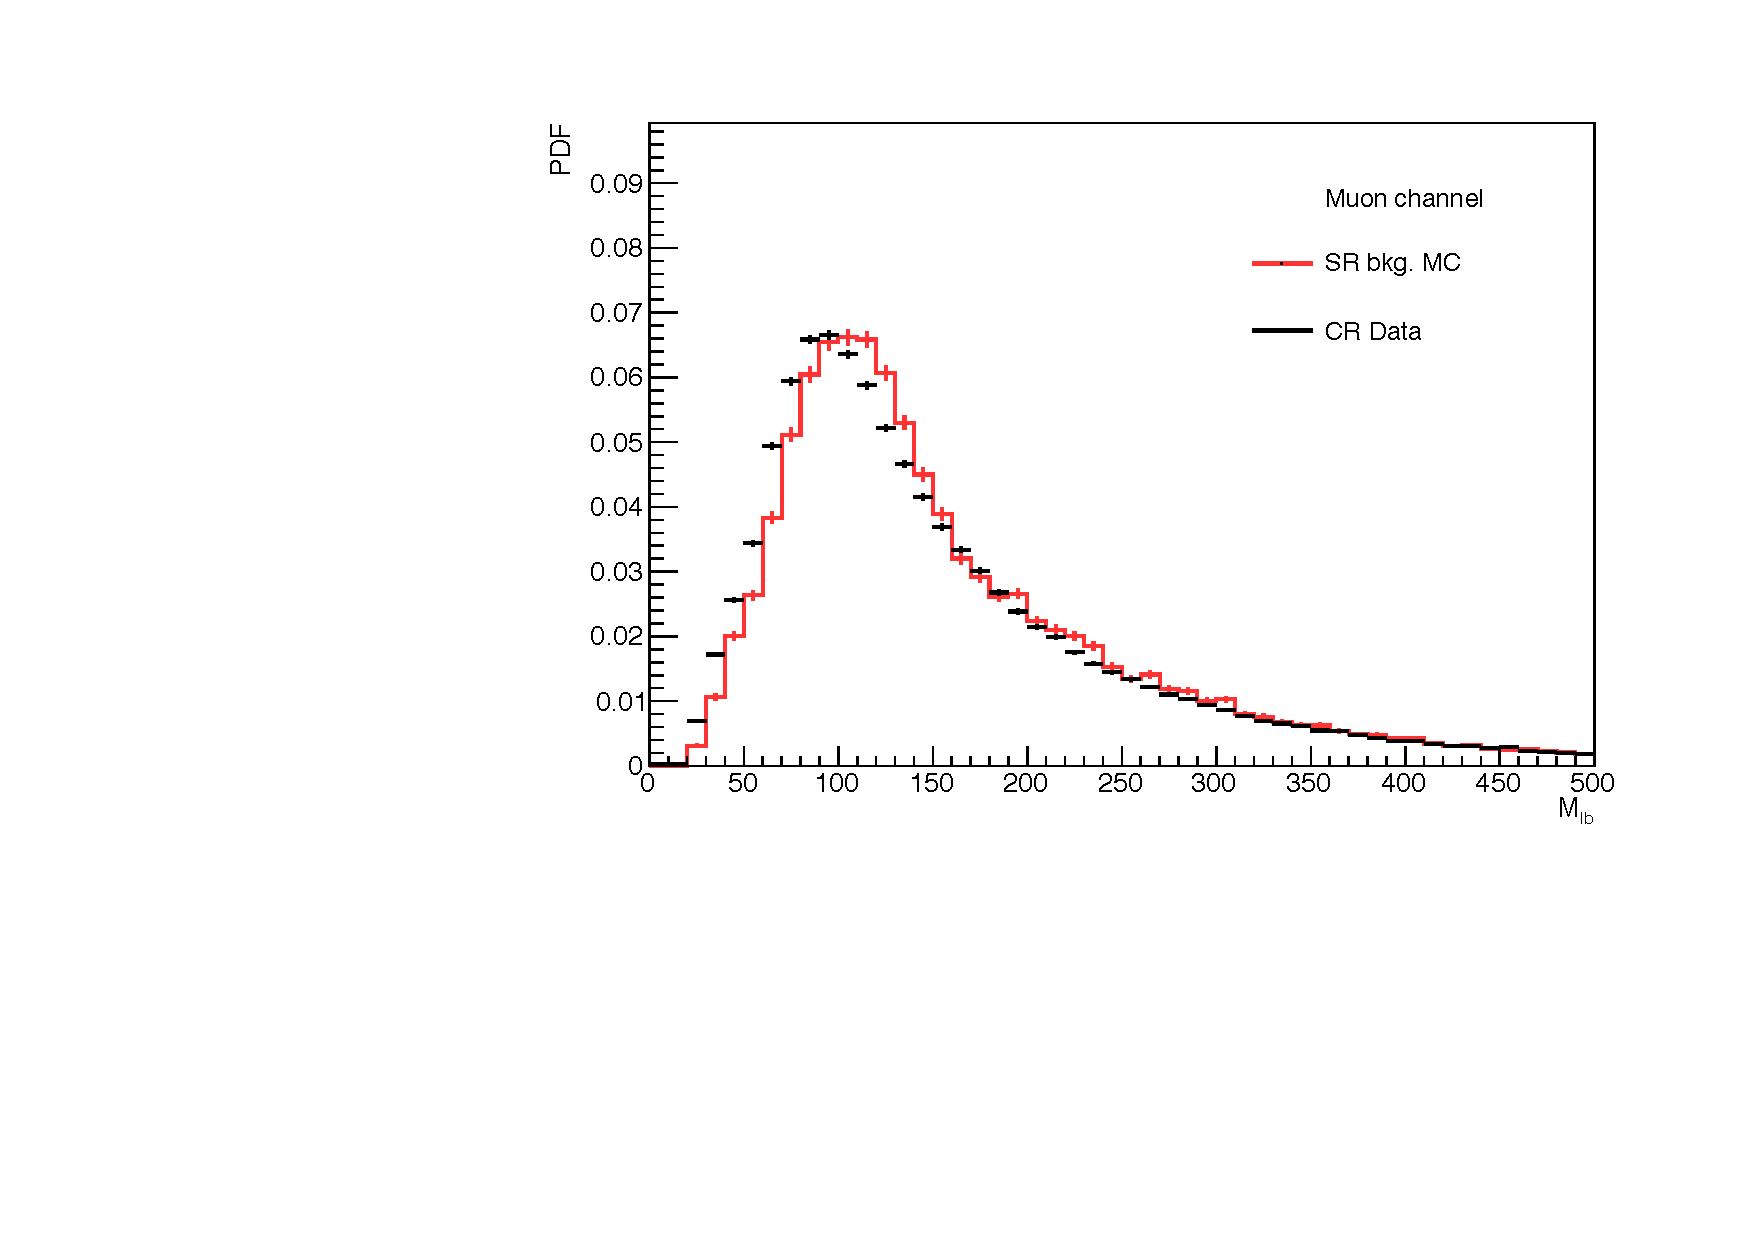
\includegraphics[width=0.45\textwidth]{Figures/BackgroundEstimation/chi2_MlbPDF_Cmp_mu.pdf}}
			\subfigure[$\chi^2_{min}$, el-ch]{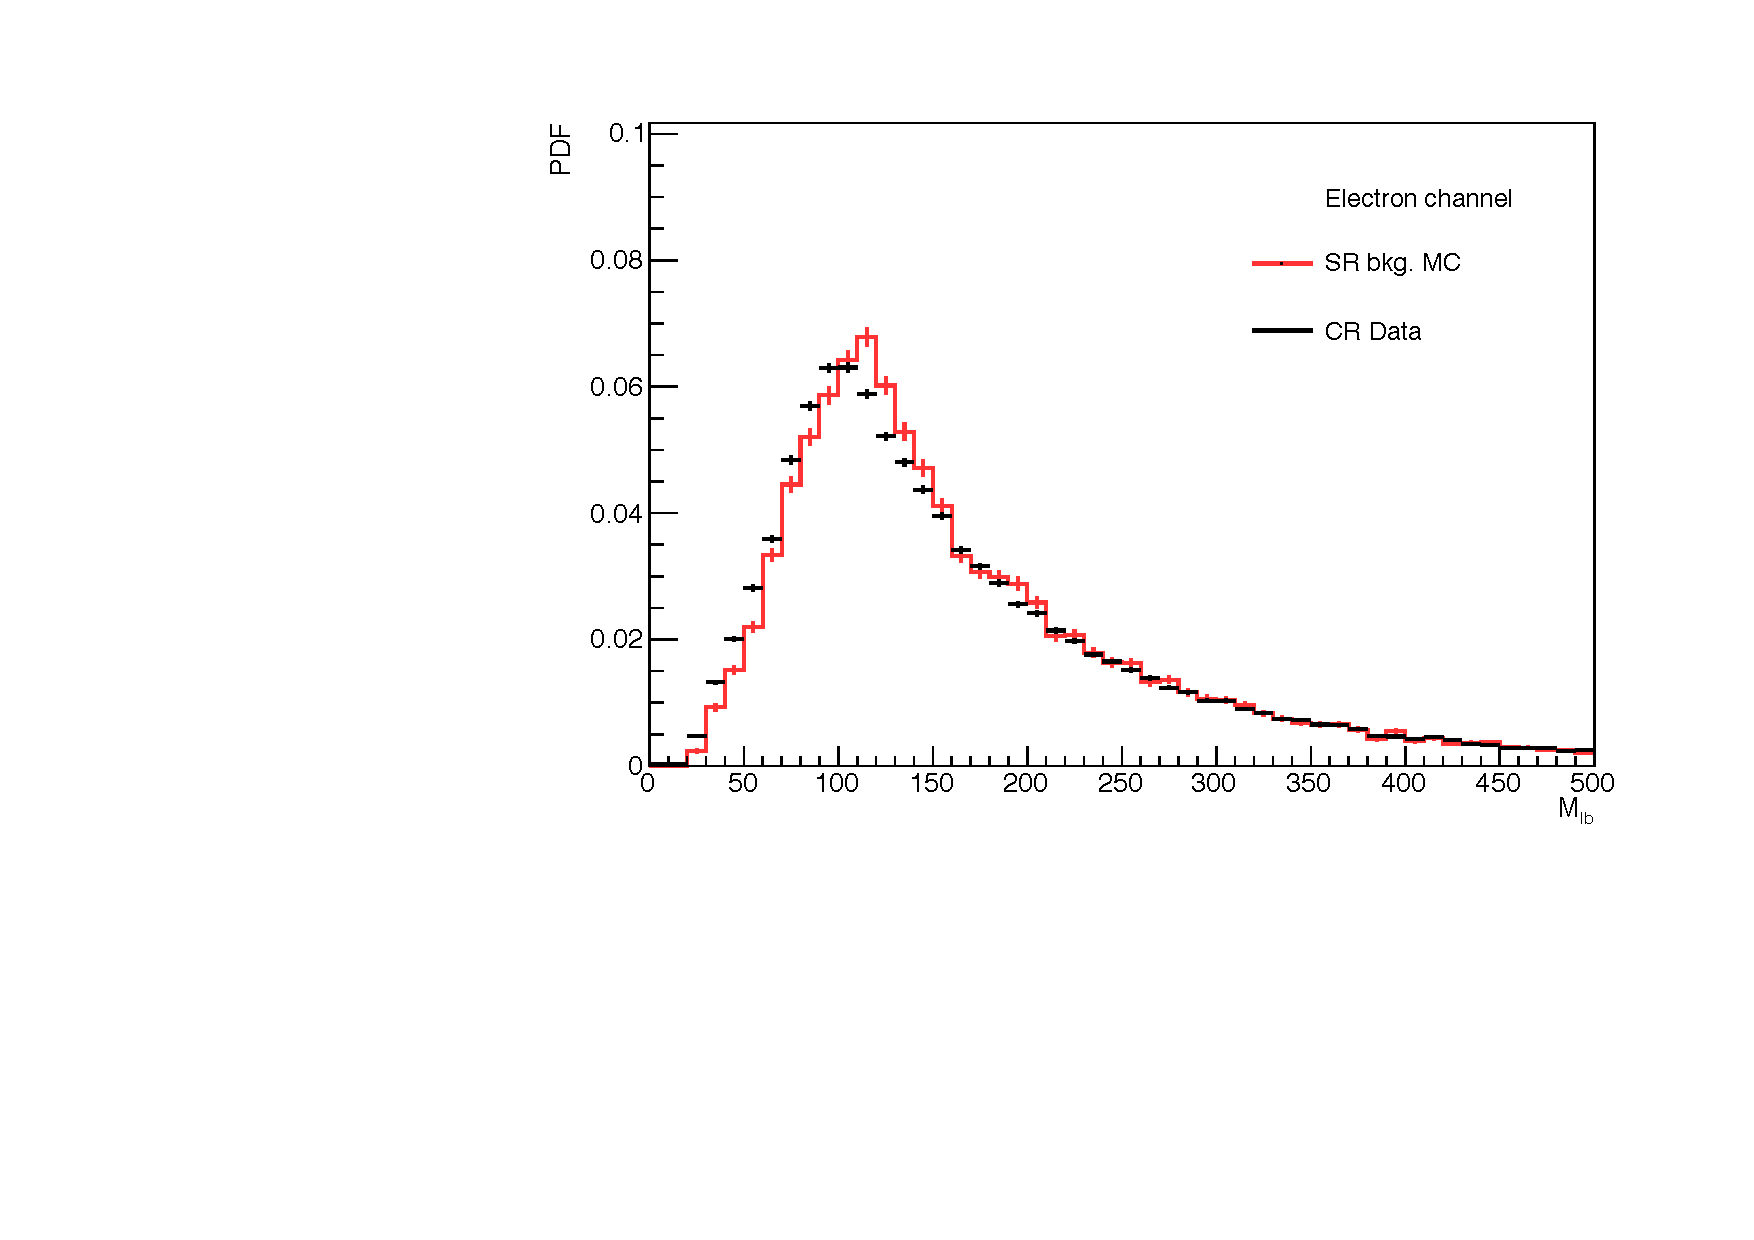
\includegraphics[width=0.45\textwidth]{Figures/BackgroundEstimation/chi2_MlbPDF_Cmp_el.pdf}}\\
		\end{figure}
		\FloatBarrier
		\begin{figure}[H]
		\centering
			\subfigure[MVA(20 variables, MLP), mu-ch]{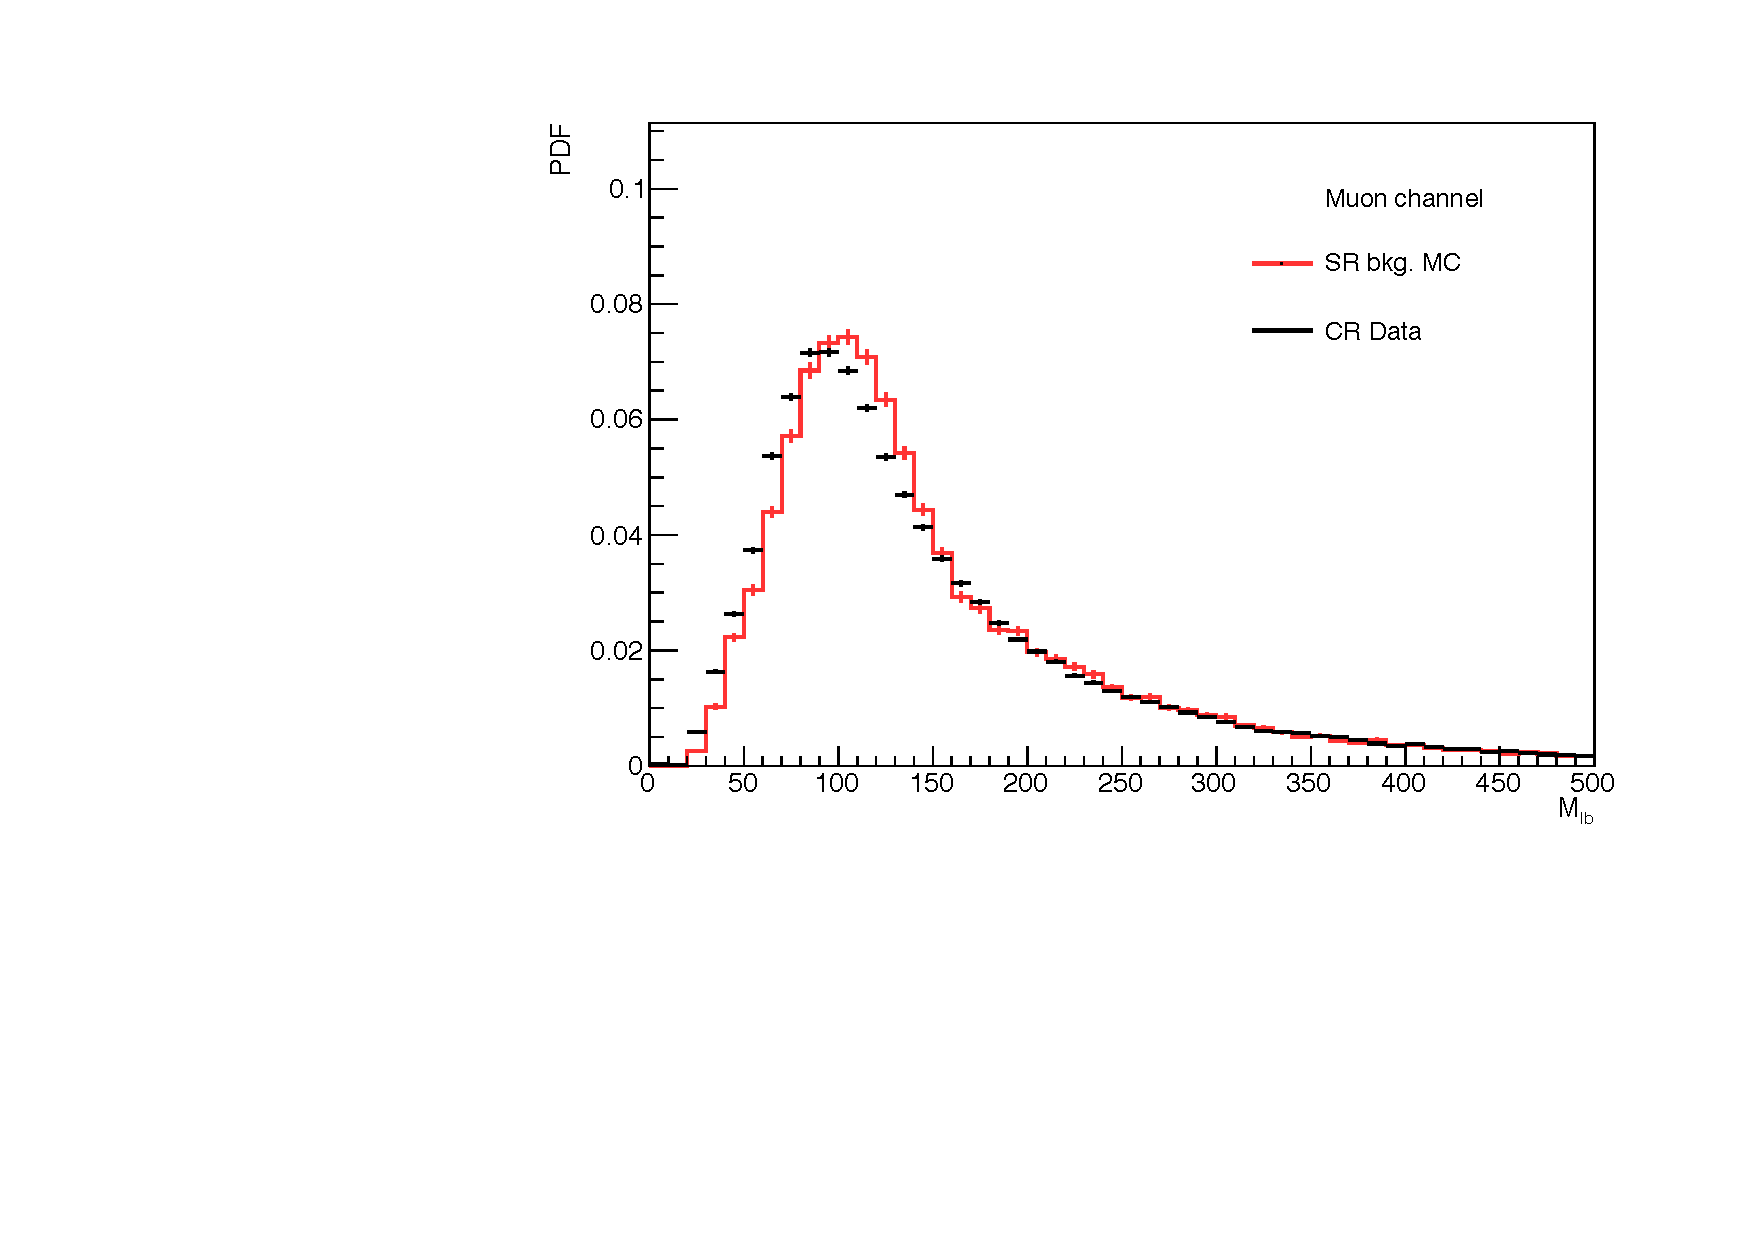
\includegraphics[width=0.45\textwidth]{Figures/BackgroundEstimation/a05_MLP_MlbPDF_Cmp_mu.pdf}}
			\subfigure[MVA(20 variables, MLP), el-ch]{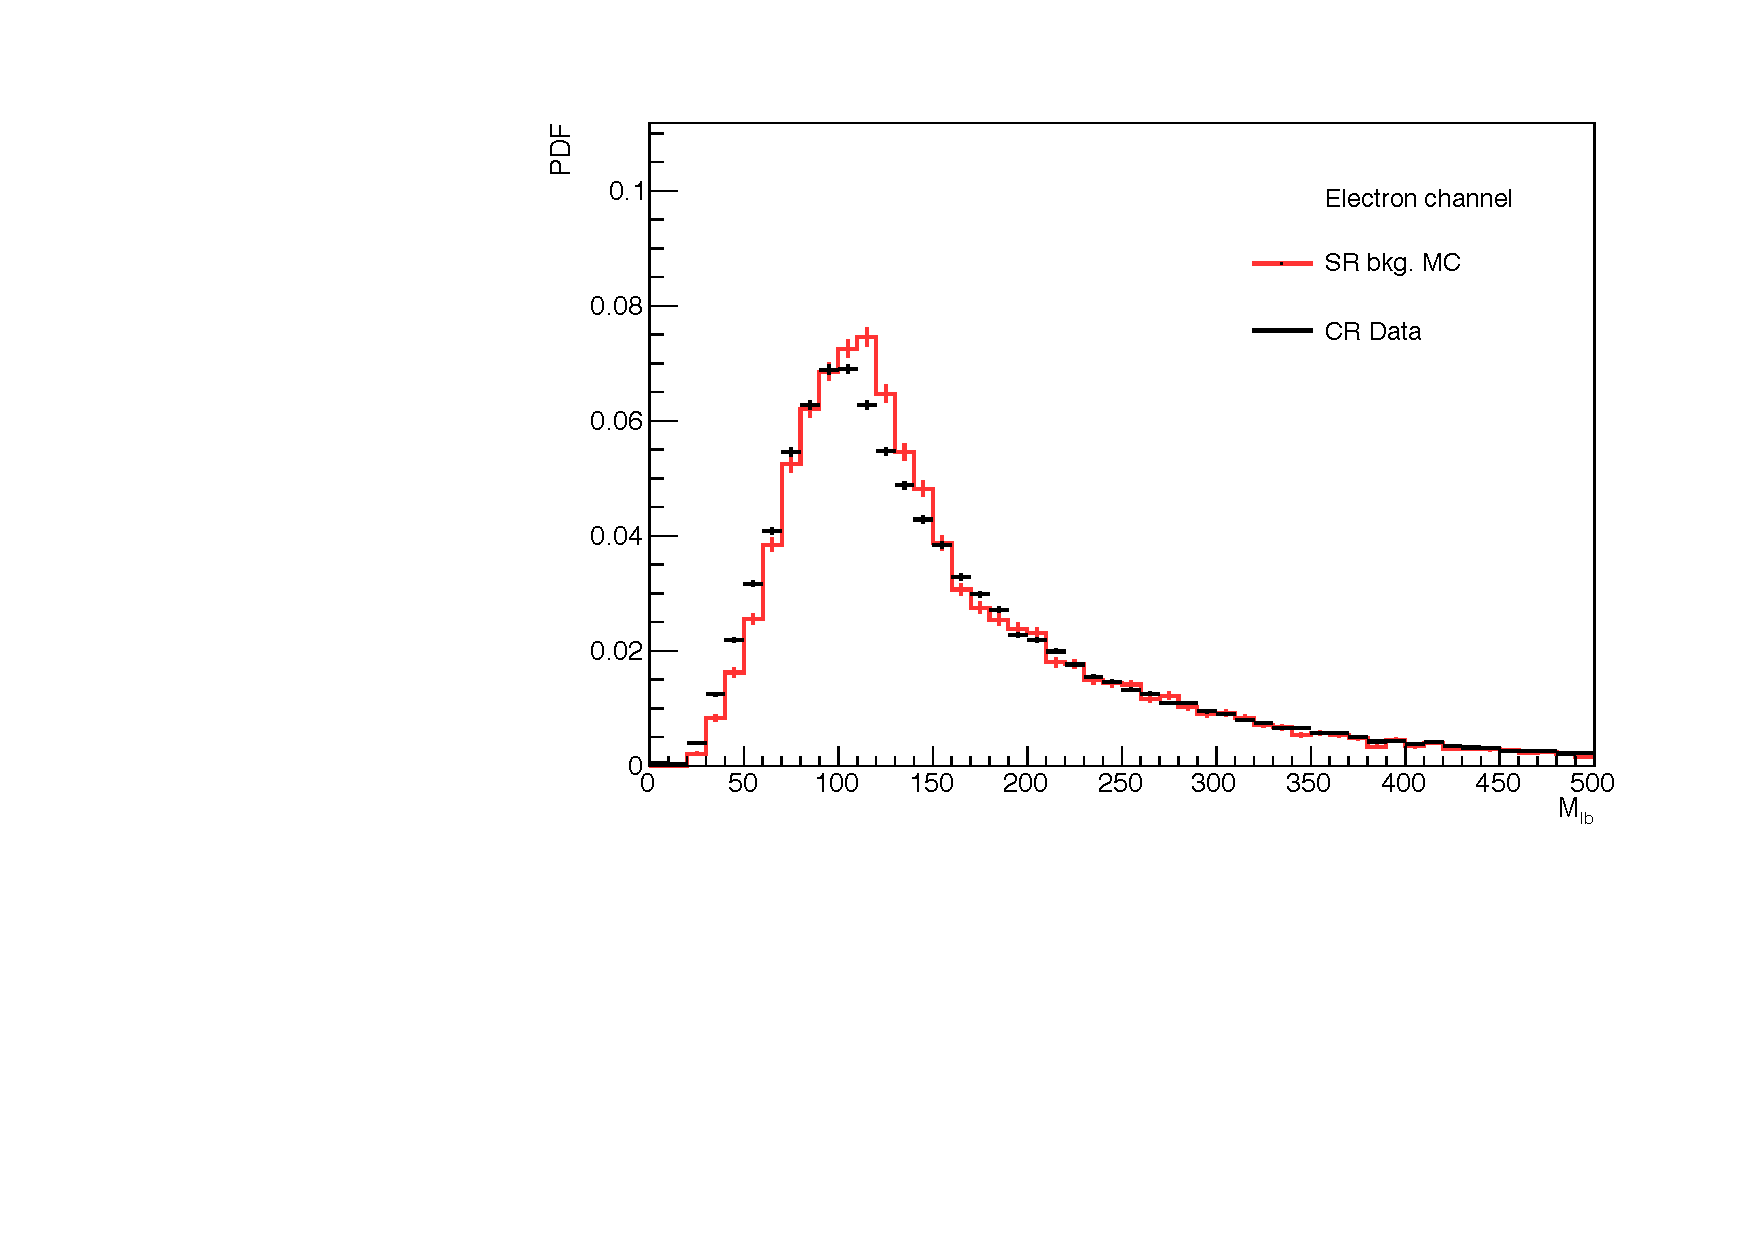
\includegraphics[width=0.45\textwidth]{Figures/BackgroundEstimation/a05_MLP_MlbPDF_Cmp_el.pdf}}\\
		\caption{Comparison of $M_{lb}$ shape between SR's background and CR's data}
		\label{BkgEst:fig:CRSR_Mlbshape}
		\end{figure}
		\FloatBarrier


	\subsection{Template Fit}
	\label{ssec:TemplateFit}

		The method $\textbf{Template Fit}$ is used to estimate background yields and subtract them in this analysis. The template in this method means a pdf(probability density function) with unvaried shape under specific variable's spectrum. Also following pdf's characteristic, the template have to be normalized(integrated area of this shape is unity). This template fit is one of general fitting with $\textbf{Maximum-Likelihood Method}$. 

		With respect to Maximum-Likelihood Method, it uses the likelihood function $\emph{L}$ and minimizes the $-2\ln{L}$ by computing resource to get the more appropriate parameters in function we want to predict. The signal and background yields in this analysis are both the target parameters in fitting. The likelihood function comes from joint pdf of N independent observation with $\emph{\textbf{X}}$ which is the set of observables, the joint pdf is Eq.\ref{eq:joint_eq}. 

		\begin{equation}
		P(X|\theta) = 􏱛 \prod_{i=1}^{N} f(X^i|\theta)
		\label{eq:joint_eq}
		\end{equation}

		 Eq.\ref{eq:joint_eq} shows the product of all i-th observation's function and the $\theta$ is the set of parameters in the pdf. When we substitute the observed data $\emph{\textbf{X}}^{\emph{\textbf{0}}}$ for variables $\emph{\textbf{X}}$, the PDF becomes the $\textbf{Likelihood function L(} \theta \textbf{)}$:

		\begin{equation}
		L(\theta) = P(X^0|\theta) = 􏱛p(N|\theta) \prod_{i=1}^{N} f(X^i|\theta)
		\label{eq:likelihood_fn}
		\end{equation}

		There are $N$ times measurements in likelihood function. Also, the $p(N|\theta)$ is usually a poisson distribution in most common case because of the common counting condition. In order to get the most appropriate parameters to match the observed data, the larger value of likelihood function $L(\theta)$, the more matched the parameters demonstrate. Therefore, the maximum $L(\theta)$ case should be the target for final decision of parameters. However, the modern technics are usually used to minimize some values, so it is turned to negative sign and being have to be minimized. On the other hand, it is convenient to calculate with addition instead of product, so doing the natural logarithm on likelihood function make it easier(Eq.\ref{eq:nature_log_L}). In conclusion, Maximum-Likelihood method minimizes the $-2\ln{L(\theta)}$ and get the fitting parameters.

		\begin{equation}
		L(\theta) \implies \ln{L(\theta)} \; \; \; \; , \; \prod_{i=1}^{N} f(X^i|\theta) \implies \sum_{i=1}^{N} \ln{L(\theta)}
		\label{eq:nature_log_L}
		\end{equation}

		In the cases that the number of observation is also the parameters and as random variables, the $\textbf{extended-likelihood function}$ is often adopted. The extended-likelihood function includes the poisson distribution $p(N|\theta)$ of Eq.\ref{eq:likelihood_fn} in. So the extended-likelihood function shows as the pattern in Eq.\ref{eq:ext_likelihood_fn}. 

		\begin{equation}
		L(\theta)_{ext} = 􏱛p(N|\theta) \prod_{i=1}^{N} f(X^i|\theta) = \frac{e^{-\mu(\theta)}\mu(\theta)^{N}}{N!} \prod_{i=1}^{N} f(X^i|\theta)
		\label{eq:ext_likelihood_fn}
		\end{equation}


		In this analysis, there are signal and background templates being pdf shapes, and the only parameters of $\theta$ set are the event numbers of signal and background($n_{S}$, $n_{B}$). Thus the extended-likelihood function of this analysis is demonstrated as Eq.\ref{eq:ext_likelihood_fn_this}. The $f_{S}$, $f_{B}$ are the fraction of signal and background. That is to say, $f_{S}$ = $n_{S}/(n_{S}+n_{B})$, $f_{B}$ = $n_{B}/(n_{S}+n_{B})$, and the $P_{S}$ and $P_{B}$ are the templates of signal and background. Also, we just fit under the $M_{lb}$ variable(oboservable), so the $X^i$ in Eq.\ref{eq:ext_likelihood_fn} is $M_{lb}$.

		
		\begin{equation}
		\begin{split}
		L(n_{S},n_{B})_{ext} = \frac{e^{-(n_{S}+n_{B})}(n_{S}+n_{B})^{N}}{N!} \prod_{i=1}^{N} f(M_{lb}^i|n_{S},n_{B}) \\
		= \frac{e^{-(n_{S}+n_{B})}(n_{S}+n_{B})^{N}}{N!} \prod_{i=1}^{N} [f_{S}P_{S}(M_{lb}^i) + f_{B}P_{B}(M_{lb}^i)] \\
		 = \frac{e^{-(n_{S}+n_{B})}}{N!} \prod_{i=1}^{N} [n_{S}P_{S}(M_{lb}^i) + n_{B}P_{B}(M_{lb}^i)]
		\end{split}
		\label{eq:ext_likelihood_fn_this}
		\end{equation}

		Eventually, in our analysis we use binned-likelihood function as the observed mode. In other words, the $i=1,2,\ldots,N$ means that input observations are the results of N bins under the observable -- $M_{lb}$ spectrum. By contrast, the unbinned-likelihood method uses event-by-event as the observation, costing too much resource and time, so it has not been used.


		\subsubsection{Fitting Result}
		\label{sssec:FittingResult}

		\begin{figure}[H]
		\centering
			\subfigure[$\chi^2_{min}$, mu-ch]{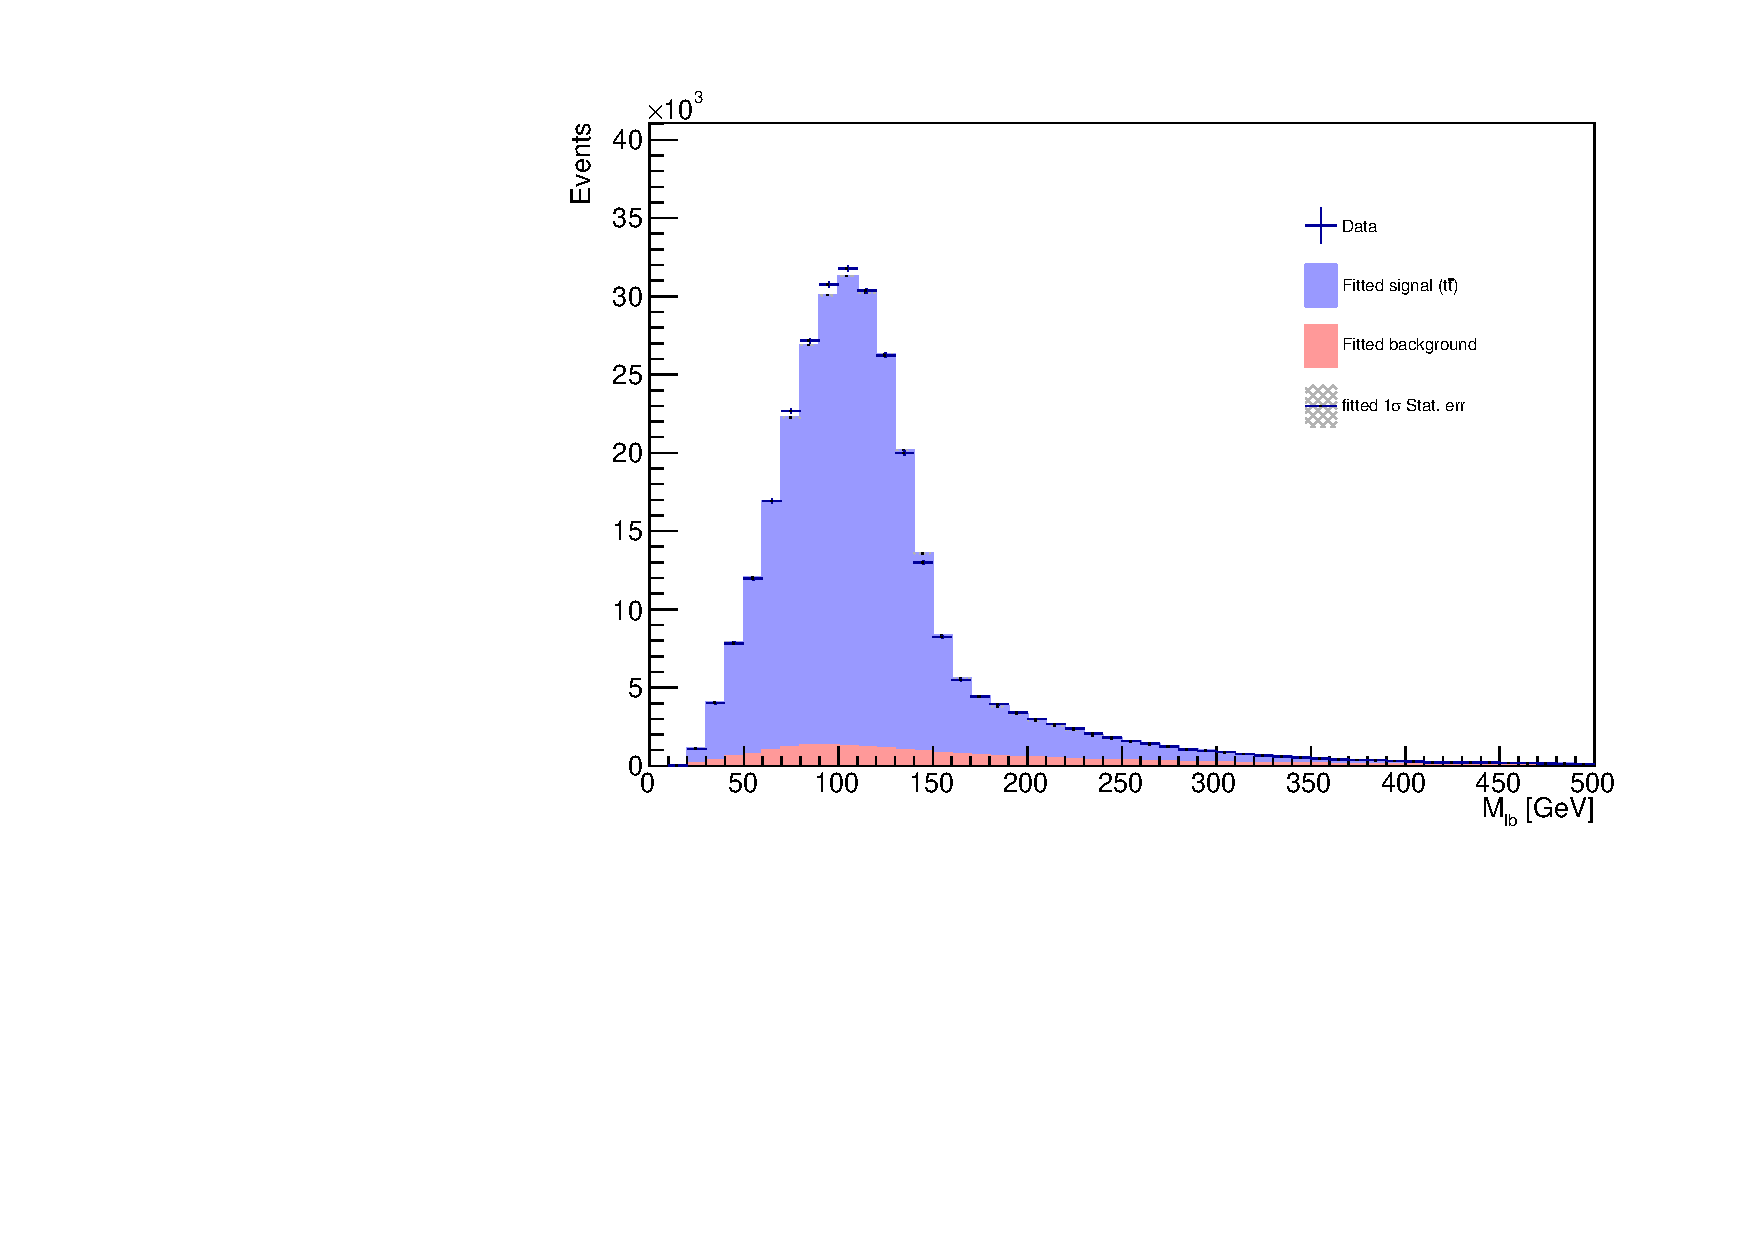
\includegraphics[width=0.45\textwidth]{Figures/BackgroundEstimation/[mu]new_chi2_fit.pdf}}
			\subfigure[$\chi^2_{min}$, el-ch]{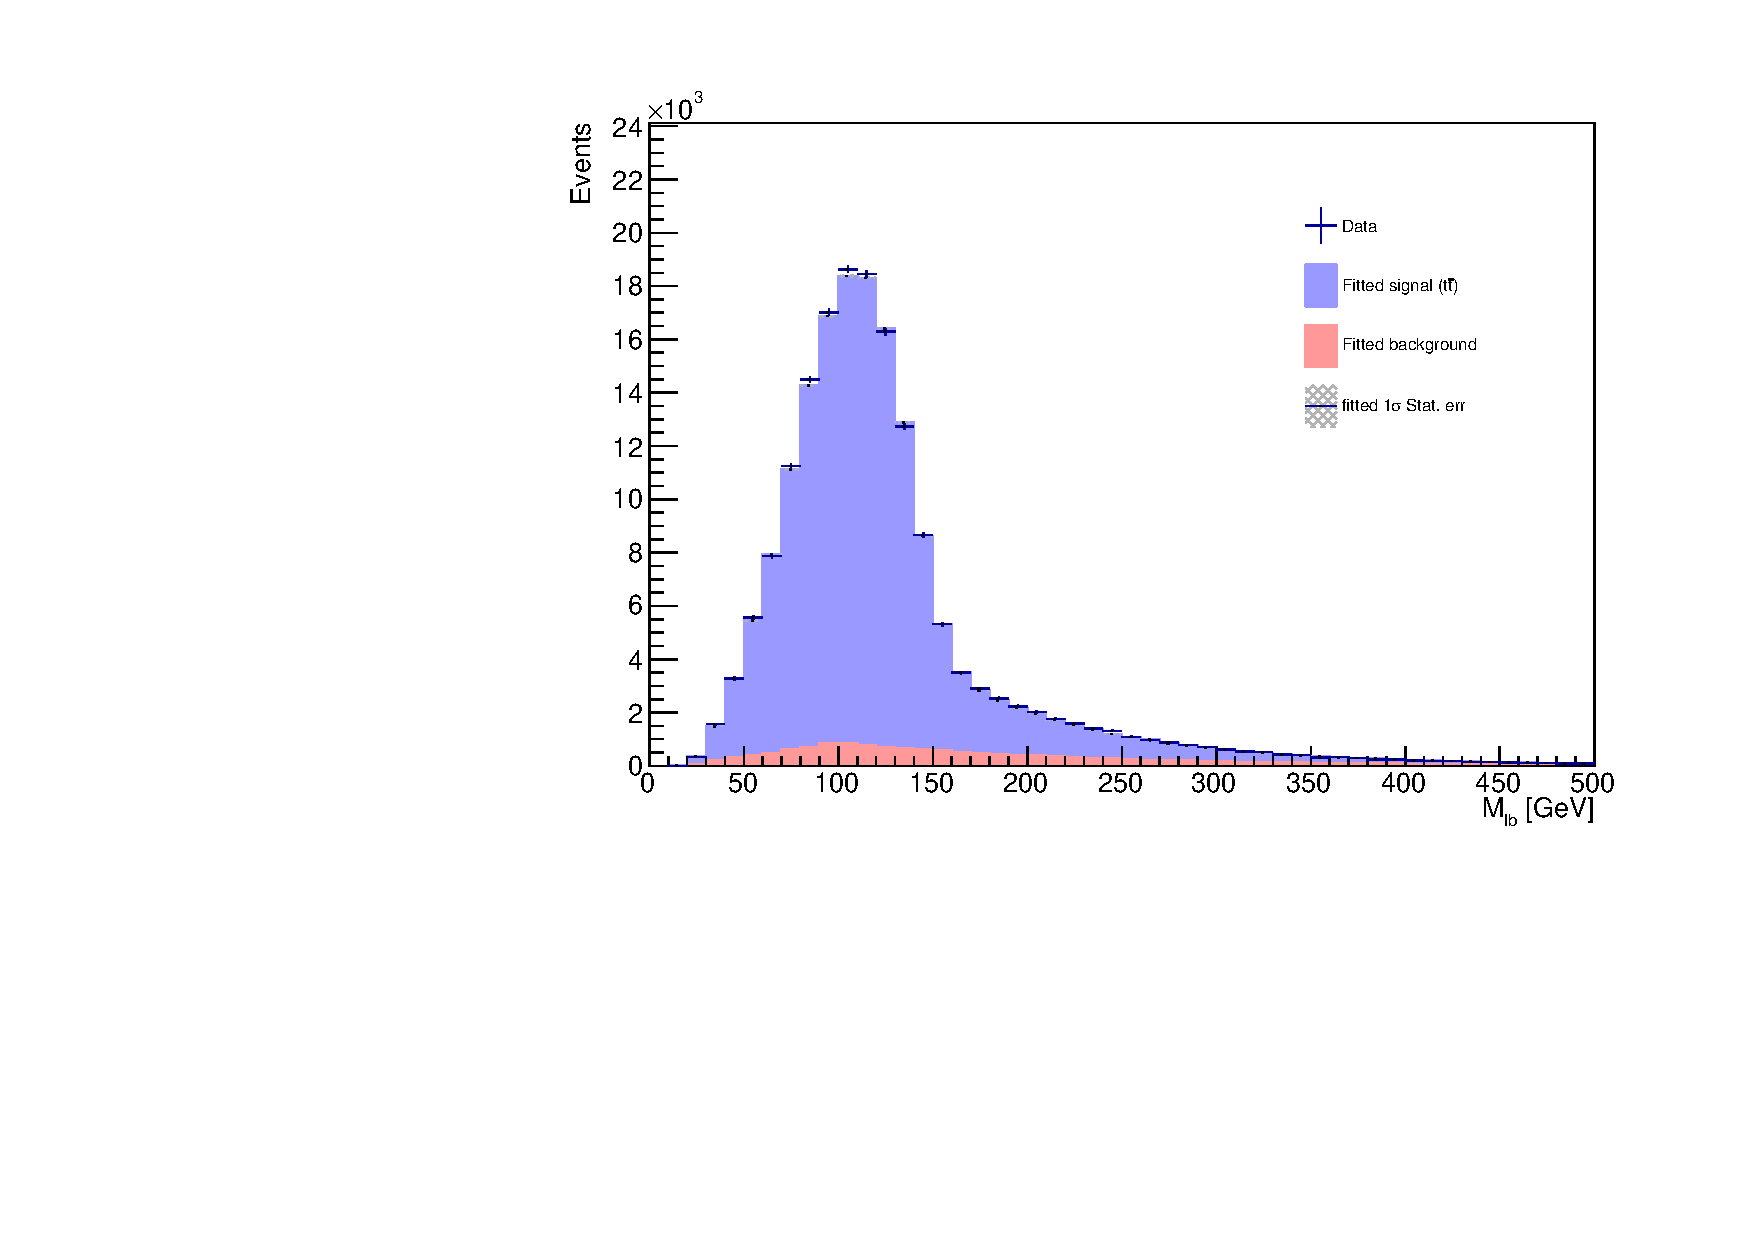
\includegraphics[width=0.45\textwidth]{Figures/BackgroundEstimation/[el]new_chi2_fit.pdf}}\\
		\end{figure}
		\FloatBarrier
		\begin{figure}[H]
		\centering
			\subfigure[MVA(20 variables, MLP), mu-ch]{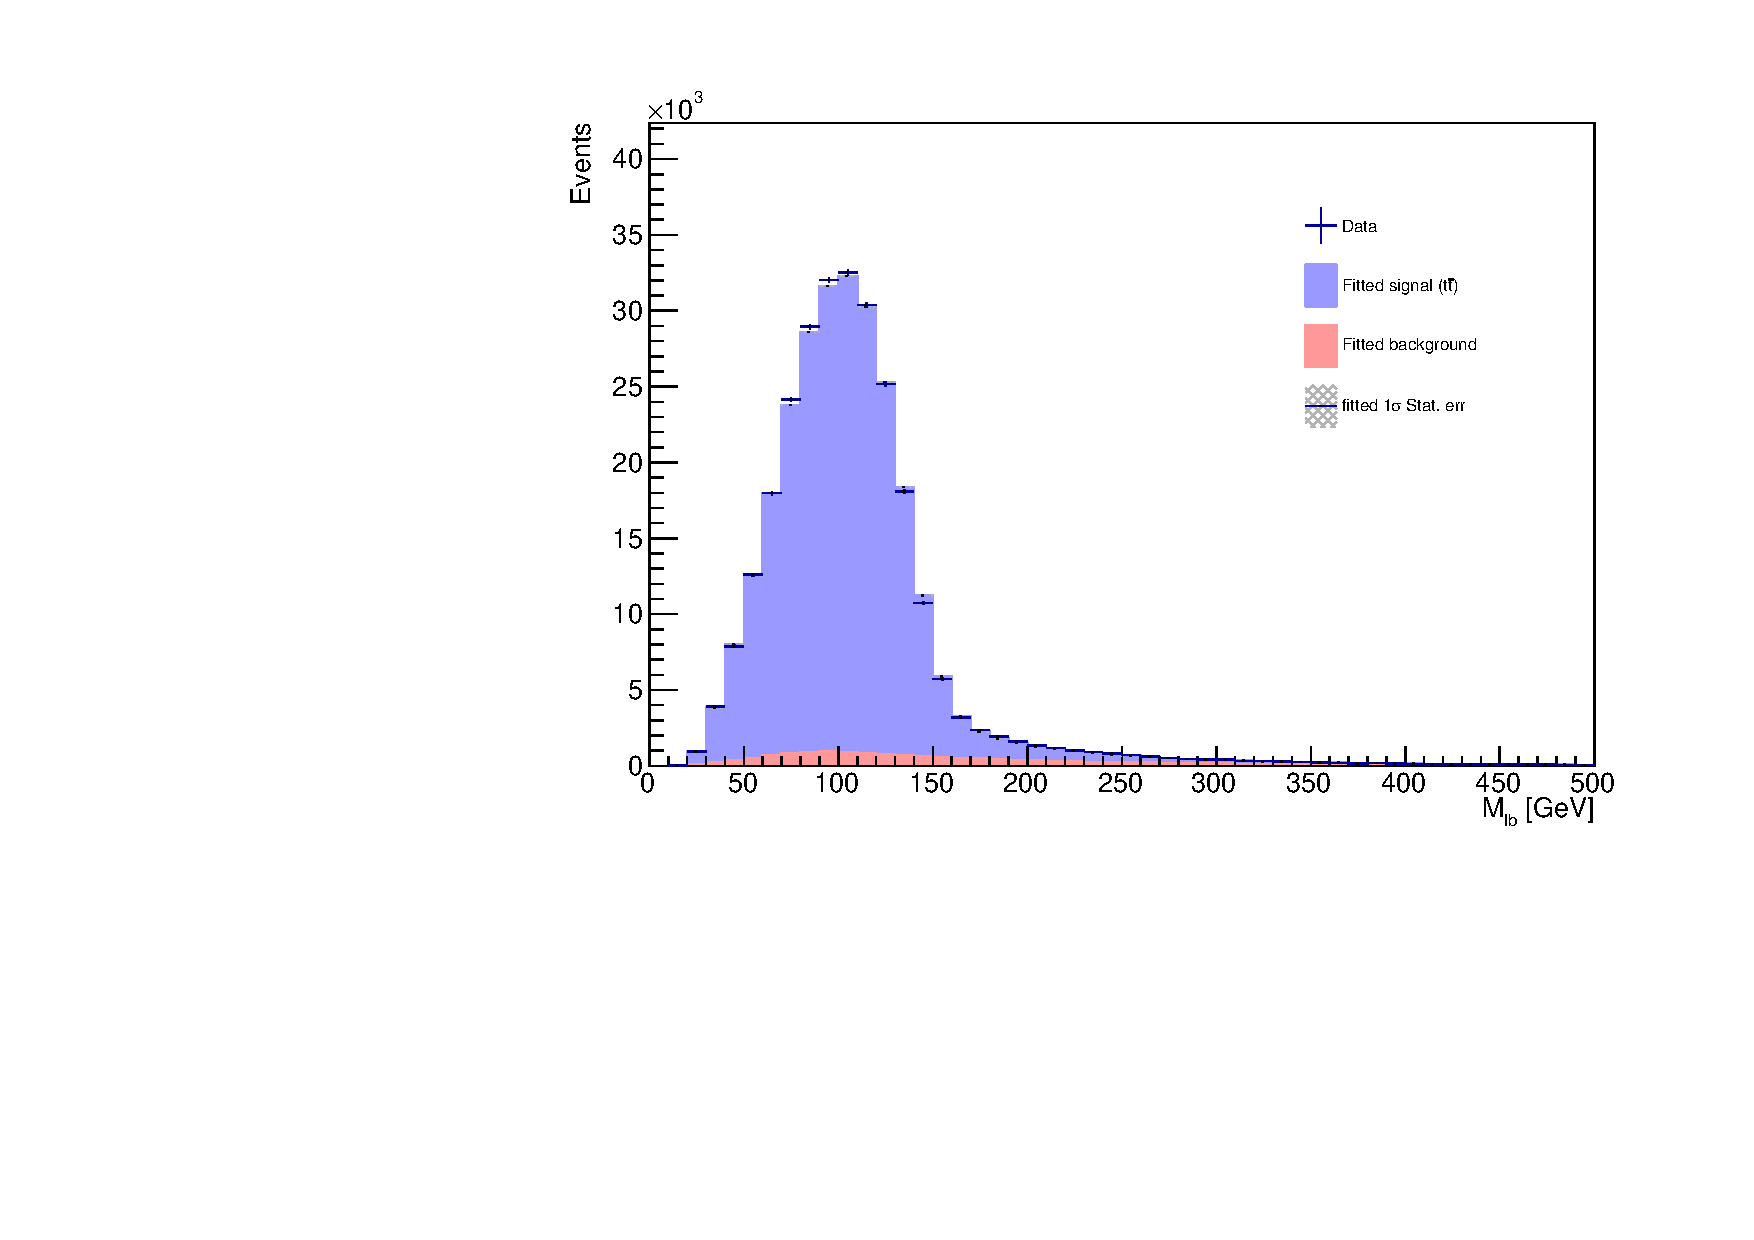
\includegraphics[width=0.45\textwidth]{Figures/BackgroundEstimation/[mu]new_a05_MLP_fit.pdf}}
			\subfigure[MVA(20 variables, MLP), el-ch]{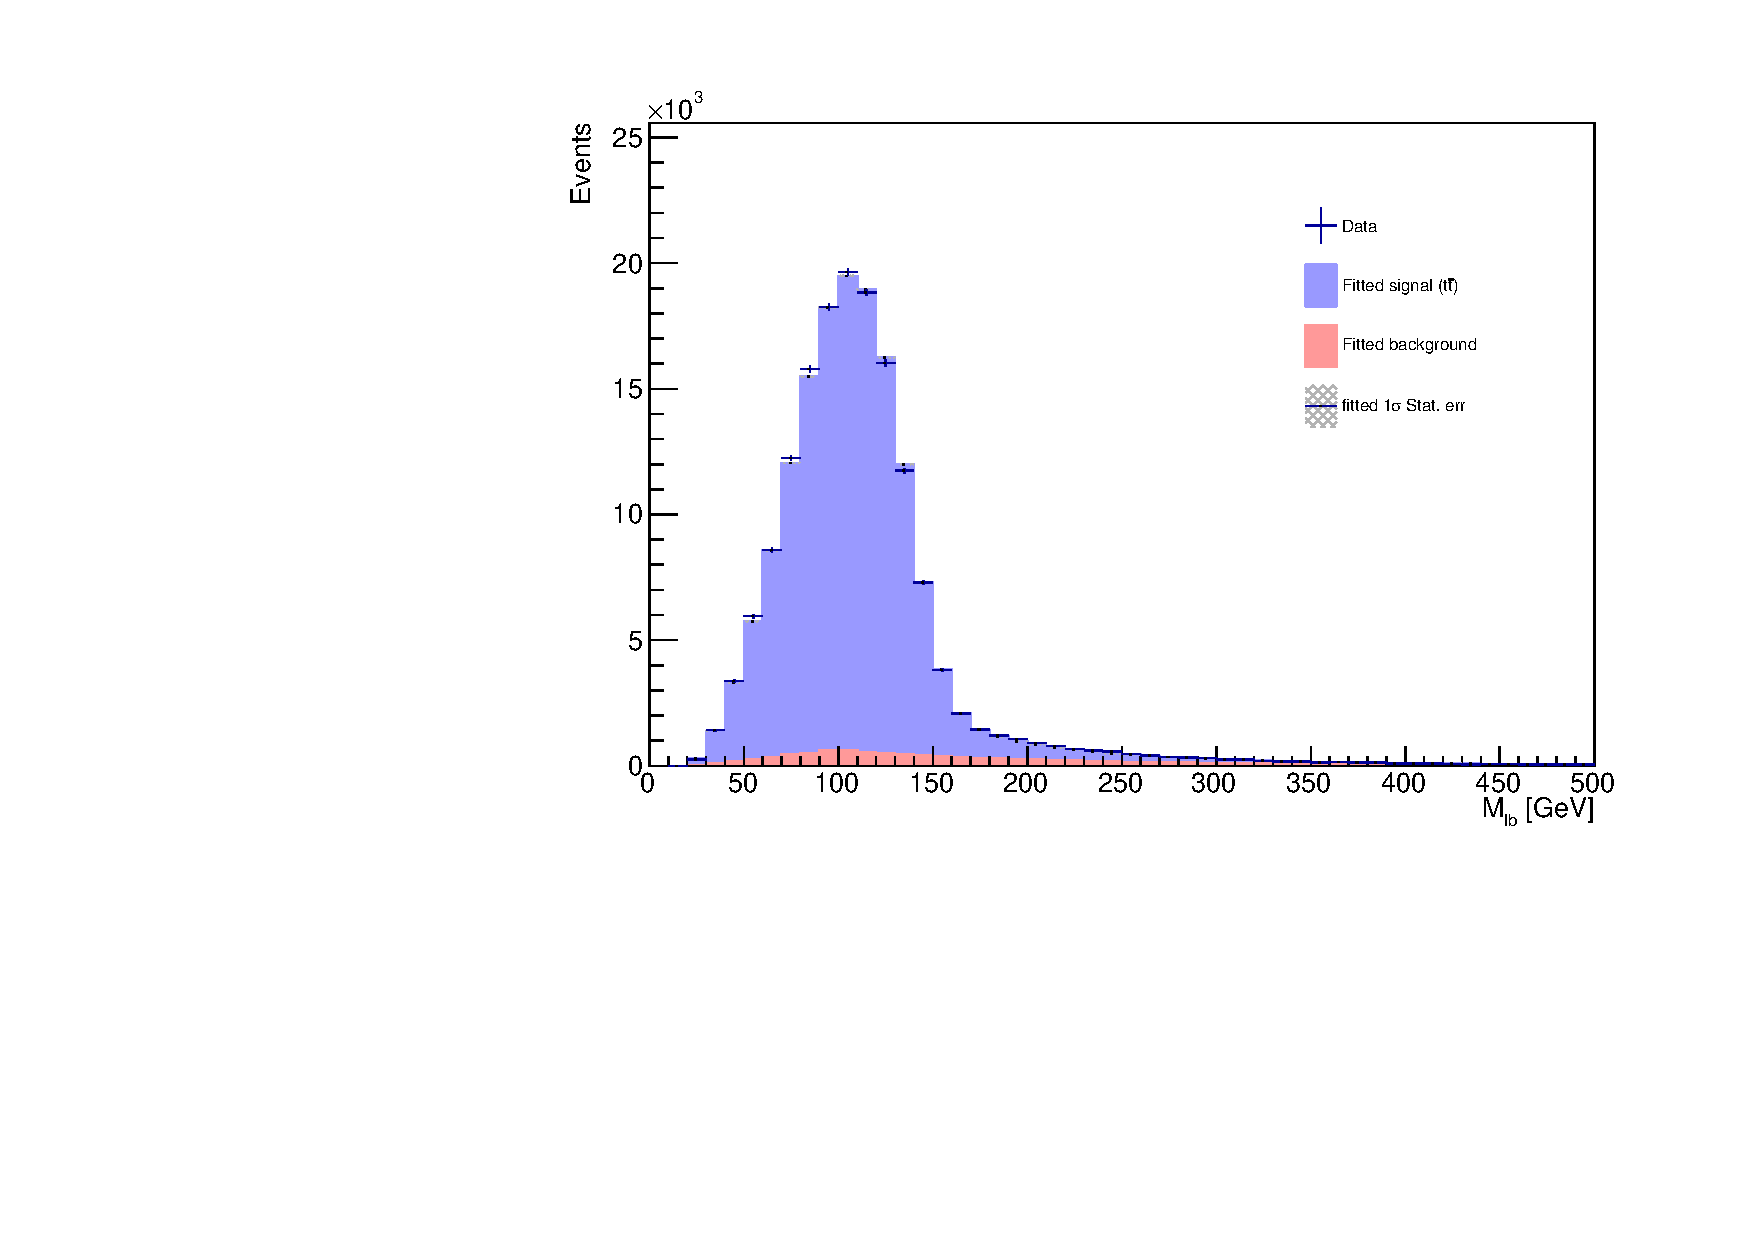
\includegraphics[width=0.45\textwidth]{Figures/BackgroundEstimation/[el]new_a05_MLP_fit.pdf}}\\
		\caption{Comparison of $M_{lb}$ shape between SR's signal and background}
		\label{BkgEst:fig:SR_sigbkg_Mlbshape}
		\end{figure}
		\FloatBarrier


		\begin{center}
		\begin{longtable}[H]{ c c c }
		\caption{Data and MC estimated events number after template fit(w/ $\chi^2_{min}, M_{lb}$ cut)} \\
		\hline
		 & Muon Channel & Electron Channel \\ 
		\hline
		 Data & 243790 & 136151 \\
		\hline
		 Expected $t\bar{t}$ & 230766 & 135600 \\
		 Expected background & 12146.9 & 5537.45 \\
		\hline
		\label{BkgEst:tb:DataMC_est_chi2}
		\end{longtable}
		\end{center}
		\FloatBarrier

		\begin{center}
		\begin{longtable}[H]{ c c c }
		\caption{Data and MC estimated events number after template fit(w/ MVA-A strategy)} \\
		\hline
		 & Muon Channel & Electron Channel \\ 
		\hline
		 Data & 245436 & 139432 \\
		\hline
		 Expected $t\bar{t}$ & 236226 & 133894  \\
		 Expected background & 8520.95 & 5102.1 \\
		\hline
		\label{BkgEst:tb:DataMC_est_MVAA}
		\end{longtable}
		\end{center}
		\FloatBarrier

		\begin{center}
		\begin{longtable}[H]{ c c c }
		\caption{Data and MC estimated events number after template fit(w/ MVA-B strategy)} \\
		\hline
		 & Muon Channel & Electron Channel \\ 
		\hline
		 Data & 272583 & 157510 \\
		\hline
		 Expected $t\bar{t}$ & 256196 & 146656 \\
		 Expected background & 15479 & 10217.6 \\
		\hline
		\label{BkgEst:tb:DataMC_est_MVAB}
		\end{longtable}
		\end{center}
		\FloatBarrier

		\subsubsection{Goodness of Fit}
		\label{sssec:GoF}

	





\FloatBarrier
